\chapter{Implementation}\label{ch:impl}
This Chapter presents the set of features that were implemented, while providing an explanation regarding their necessity and specific details about how they were created.


\section{Nested features}
The task that had the highest priority was to make it possible to handle nested features, a functionality that had not been supported earlier, as mentioned in \textcite{Jecdar:2019}. The first version of \jecdar was able to handle composition and conjunction of simple automata (e.g., Administration || Machine || Researcher or HalfAdm1 \&\& HalfAdm2), but nesting such features was out of its scope.

We understood that handling such an issue would require changes in our data structures. A state used to be represented as a vector of locations (where each location would correspond to an automaton) and a zone. When trying to retrieve the next possible transitions that can be taken from a certain state, we would have to gather all the transitions that can be taken by each subcomponent. With a flat structure of the current location, this is hard to achieve, as we no longer know which part of the location corresponds to which transition system.

\begin{figure}
  \centering
  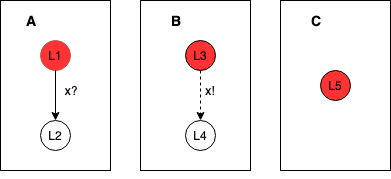
\includegraphics[scale=0.7]{figures/nestedLoc.png}
  \caption{(A || B) || C}
  \label{fig:nestedLoc}
\end{figure}

Figure \ref{fig:nestedLoc} illustrates this problem. It shows a composition between another composition (A || B) and a simple automaton, C. Note that, for simplicity, only the relevant parts of the automata are displayed. The red locations represent the current location. Being in the state consisting of locations L1, L3 and L5, we would like to know what transitions can be taken with the action x. If our location was simply represented as a vector of locations, we would not know which part of it we need in order to fetch the next transitions from (A||B) and from C.

\begin{figure}
  \centering
  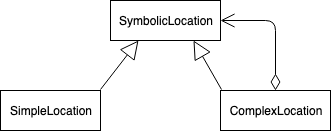
\includegraphics[scale=0.7]{figures/nestedness.png}
  \caption{Structure of the SymbolicLocation class}
  \label{fig:nestedness}
\end{figure}

We solved this issue by refactoring our location vector into what we call a "symbolic location". This new data type is represented by an abstract class, with two classes inheriting from it, as shown in Figure \ref{fig:nestedness}. A SymbolicLocation can be either a SimpleLocation or a ComplexLocation. A SimpleLocation is simply a wrapper for a regular Location, while a ComplexLocation can have many SymbolicLocations.

\begin{figure}
  \centering
  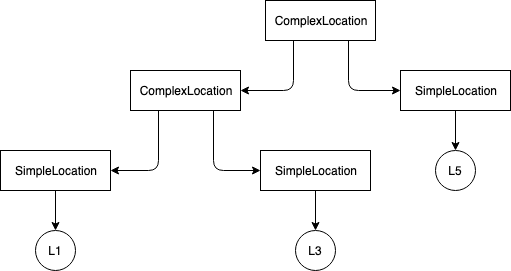
\includegraphics[scale=0.7]{figures/symbolicLoc.png}
  \caption{Tree representation of a location}
  \label{fig:symbolicLoc}
\end{figure}

This approach allows us to store locations as tree structures than can be built in a recursive fashion. Figure \ref{fig:symbolicLoc} shows how the location from (A || B) || C is represented in terms of the new data structure.

\begin{figure}
  \centering
  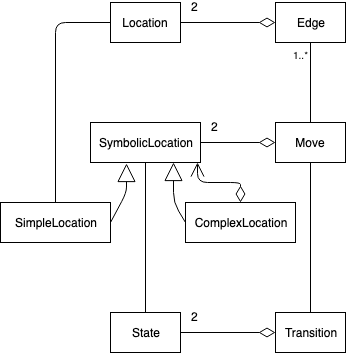
\includegraphics[scale=0.7]{figures/umlTransitions.png}
  \caption{Class diagram}
  \label{fig:umlTransitions}
\end{figure}

Moreover, if we previously used to retrieve outgoing edges from a location, after introducing symbolic locations we discovered the need to create a corresponding abstraction for outgoing edges from a symbolic location. We gave this new concept the name of "Move", and its purpose is to connect two symbolic locations through a vector of edges. This way, we can get the moves that can be taken from each symbolic location of a certain state and then aggregate them in order to build a transition. Figure \ref{fig:umlTransitions} presents the correlation between states, symbolic locations and locations and the one between transitions, moves and edges.


\section{Addition of strictness} \label{sec:strictnessFix}

As explained in \textcite{Jecdar:2019}, since transition systems can be infinite due to an infinite amount of states given by time being continuous, we must use a symbolic representation of states in order to achieve finiteness. A common approach is to make use of zones, which contain intervals for each clock, and this is also the approach that we chose. We represent zones through DBMs (difference bound matrices), which allow us to specify the upper bound on the difference between each two clocks. 

\begin{figure}
  \centering
  \includegraphics[scale=0.7]{figures/strictness.png}
  \caption{Conversion from actual DBM to internal representation}
  \label{fig:strictness}
\end{figure}

The DBM library allows us to construct such constraints and to specify their strictness (< or $\leq$). The value and its strictness are encoded in each constraint. We noticed that we were building DBMs incorrectly, as by default all our constraints were non strict and we used to modify the values in order to match the strictness (e.g., $x < 7$ would be turned into $x \leq 6$, which means that the values from the interval (6, 7) would be omitted).

In Figure \ref{fig:strictness} we show an example of an actual DBM and how the previous version of \jecdar used to adjust the values according to the strictness and then convert it into the library's internal representation. We also illustrate the correct representation that we now achieve by eliminating the adjustment and encoding each constraint according to its strictness.

\section{XML Parser}

The first version of \jecdar had a JSON parser for the models created with \ecdar 2.x. In order to automate our tests as much as possible, it was important to avoid creating test cases manually. The most suitable approach that we found was to create models in \ecdar 2.x, which can later be parsed into our internal data structures that the tests can be run on. We would run different queries on these models and use the results to infer the expected output of each test. Our reason for choosing \ecdar 2.x was the fact that it was our intention to integrate \jecdar with the new GUI at a later point, so it made sense to use it for creating models and verifying properties of them.

After experiencing questionable results when running certain queries, we decided to check whether \ecdar 0.10 would provide us with different outputs. As expected, \ecdar 0.10 gave the same results, and that makes sense since both versions are using the same engine behind the scenes. However, \ecdar 0.10 would also display handy error messages. (e.g., the reason why a refinement holds or does not hold).

Henceforth, we made the decision to continue creating and testing models in \ecdar 0.10 and for that purpose we found it useful to create an XML parser as well. 

This parser is implemented in a similar way to the JSON one. It uses a library in order to simplify the task and to reduce the chances of making mistakes. The parsing is performed by taking a specific XML file and operating on the nodes corresponding to the automata. The result is a list of automata that together make up a model.

Moreover, since we now support models in XML format as well, we introduced one additional thing. As mentioned in \textcite{Jecdar:2019}, we have several commands that can be used for communicating with \jecdar from the terminal. The "-rq folderPath query query..." command, which runs one or more queries, given the path of the model, has been modified with the addition of an extra flag to indicate whether the model is in JSON or in XML format. The reason for doing is so that the controller can decide which parser it should use. In order to run such a command, "-rq" must be typed, followed by either "-json" or "-xml", followed by the actual queries.

\section{Determinism check} \label{sec:implDeterm}
According to \textcite{David:2010}, the specification theory was defined to be applied on deterministic TIOTS, where the following applies: for all $a \in \Sigma \cup \mathbb{R}_{\geq 0}$ whenever $s\xrightarrow{a}^S s'$ and $s\xrightarrow{a}^S s''$ we have $s' = s''$. Without this property, one would not be able to tell which edge has to be taken for an action. Therefore, a determinism must be ensured for each of the automaton and is considered an implicit prerequisite for any further application of features on that automaton.

To check for the determinism property of an automaton, one must ensure there does not exist a non-deterministic choice on an action (edge) at any location of the automaton. The Algorithm \ref{alg:isDeterministic} outlines the general implementation design for the determinism check.

\begin{algorithm}
\caption{Algorithm to verify determinism of automaton}
\label{alg:isDeterministic}
\begin{algorithmic}[1]
\Function{isDeterministic}{}
\State $Passed \gets \{\}$ 
\State $Waiting \gets \textsc{getInitialState()}$
\While{$(Waiting.hasNext)$}
    \State $state \gets Waiting.\textsc{pop}()$
    \State $passed.\textsc{add}(state)$
    \ForAll{$action$ in $actions$}
        \State $trans \gets \textsc{GetNextTransitions}(state, action)$
        \If{($\textsc{CheckMovesOverlap}(trans)$)}
            \State \textbf{return $false$}
        \Else
        \State $targets \gets (tran::\textsc{getTarget}) \notin passed $
        \State add $targets$ to $Waiting$
        \EndIf
    \EndFor
\EndWhile
\State
\State \textbf{return $true$} 
\EndFunction
\end{algorithmic}
\end{algorithm}

The idea is to check every reachable location of the automaton, but do that only once. For that, \textit{passed} and \textit{waiting} lists are used. Then for each location in the \textit{waiting} list the following applies: a) the location is moved to the \textit{passed} list, b) for each action, present in the signature of the automaton, the possible transitions are acquired, c) actions are checked for determinism (Line 9). As soon as at least a single instance of non-determinism is encountered the algorithm reports determinism to have failed (Line 10). 

Algorithm \ref{alg:moves-overlap} shows the logic behind the \textsc{CheckMovesOverlap} method. The idea behind the verification of an arbitrary amount of transitions for their "overlapping" lies in ensuring there is no intersection between all possible combinations of two transitions.

\begin{algorithm}
\caption{Algorithm to check if transitions overlap}
\label{alg:moves-overlap}
\begin{algorithmic}[1]
\Function{CheckMovesOverlap}{$trans$}
\If{($trans.size < 2$)}
    \State \textbf{return $false$};
\EndIf
    \For{($i\gets 0; i < trans.size; i++$)}
        \For{($j\gets i+1; i < trans.size; i++$)}
        \If{(trans[i].targetLoc = trans[j].targetLoc)}
        \If{(trans[i].\textsc{hasEqualUpdates}(trans[j])}
        \State \textbf{continue}
        \EndIf
        \EndIf
        \State $zone1 \gets$ trans[i].targetLoc.invZone
        \State $zone2 \gets$ trans[j].targetLoc.invZone
            \If{(\textsc{intersect}($zone1, zone2$))}
            \State \textbf{return $true$}
            \EndIf
        \EndFor
    \EndFor
\State
\State \textbf{return $false$}	
\EndFunction
\end{algorithmic}
\end{algorithm}

In principle, a single existing transition cannot create non-determinism (Lines 2-3). For a larger amount of transitions, the algorithm takes a look at every possible pair of transitions without considering the same pair more than once. Note that if a considered pair of transitions leads to the same target location and the updates (resets) of those two transitions are identical it should be considered a deterministic pair and not checked for intersection (Lines 6-8). In other words, even if two transitions lead to the same location, but their updates (resets) differ, they may create a non-deterministic choice in terms of zones for clocks if these transitions overlap.

Next, for each pair the intersection of zones is checked and if one exists then the algorithm reports non-determinism. This algorithm eliminates the problem present in \ecdar 0.10 which was described in Section \ref{sec:determBug}.

\section{Consistency check}

The determinism check is a prerequisite for the next feature implemented - consistency check. In fact, all automata must first pass the determinism check before being eligible for any further computations.

The Algorithm \ref{alg:check-consistency} is suitable for checking two types of consistency: least fixpoint consistency and full consistency, both of which were mentioned in Section \ref{sec:minConsistency}. The type of consistency to be checked is determined by the boolean variable \textit{canPrune} that is passed as an argument to the \textsc{CheckConsistency} method together with the \textit{state} from which the consistency check should begin, normally being the initial state.

This algorithm has a recursive nature and avoids loops in the structure of the automaton by maintaining the list of $passed$ states. Any state that is checked for consistency will either be added to the \textit{passed} list or return \textit{true} if the state has been already explored (Lines 2-4). 

\begin{algorithm}
\caption{Algorithm to check consistency}
\label{alg:check-consistency}
\begin{algorithmic}[1]
\Function{CheckConsistency}{$state, canPrune$}
\If{($state \in passed$)} 
\State \textbf{return} true;
\EndIf
\State add $state$ to $passed$
    \ForAll{$action$ in $inputs$}
    \State $trans \gets \textsc{GetNextTransitions}(state, action)$
        \ForAll{$tran$ in $trans$}
            \If{($\neg$\textsc{CheckConsistency}($tran.Target, canPrune$))}
            \State \textbf{return $false$};
            \EndIf
        \EndFor
    \EndFor
    \State
    \If{($canPrune$ and $state.\textsc{CanDelayIndefinitely}$)}
    \State \textbf{return $true$}
    \EndIf
    \State
    \ForAll{$action$ in $outputs$}
        \State $trans \gets \textsc{GetNextTransitions}(state, action)$
        \ForAll{$tran$ in $trans$}
            \State $isConsistent \gets \textsc{CheckConsistency}(state, canPrune)$
            \If{($consistent$ and $canPrune$)}
            \State \textbf{return $true$}
            \EndIf
            \If{($\neg consistent$ and $\neg canPrune$)}
            \State \textbf{return $false$}
            \EndIf
        \EndFor
    \EndFor
    \State
    \If{($\neg canPrune$)}
        \If{($outputExisted$)}
        \State \textbf{return $true$}
        \Else
        \State \textbf{return} $state.\textsc{CanDelayIndefinitely}$
        \EndIf
    \EndIf
    
\State
\State \textbf{return $false$}	
\EndFunction
\end{algorithmic}
\end{algorithm}

Lines 5 to 9 handle all the outgoing input edges from the current state. As mentioned in Section \ref{sec:minConsistency}, inputs cannot be assumed to never be received as they depend on the unpredictable environment. Therefore regardless of being allowed to prune inconsistent parts of the automaton or not, the targets of those input edges must always be checked for consistency. If the target state of at least one input edge appears to be inconsistent, the entire check of consistency returns \textit{false} (Lines 8-9).

Interestingly, with the least fixpoint consistency it suffices to find the earliest state that satisfies the property of independent progress and simply prune the rest. In such cases, when the consistency check is allowed to prune, the two lines 11 and 12 are executed. The algorithm returns \textit{true} if independent progress property is satisfied by the state being able to delay indefinitely.

If the state was not able to delay indefinitely or the pruning was not allowed, the algorithm proceeds to checking all the outgoing output edges. Each outgoing edge is checked for consistency by performing a recursive call and the boolean result is stored in the \textit{isConsistent} variable (Line 17). In the case of being allowed to prune states, having found at least a single consistent state suffices for the entire consistency check to return $true$ (Lines 18-19). On the other hand, not being able to prune states and having found at least one inconsistent state reached by an output edge means not satisfying the consistency check (Lines 20-21).

After having checked both input and output edges of the state there is some logic left for cases of computing full consistency. If an output edge existed at that state and we have not found any inconsistent states reached by any edges, the algorithm is safe to report the automaton being consistent(Lines 24-25). However, if no outputs existed, the only way to ensure the independent progress property becomes the possibility of the state to delay indefinitely (Lines 26-27). 

Finally, if by the very end of the algorithm none of the return statements were triggered, it means that no states managed to satisfy the property of independent progress and, therefore, the algorithm terminates.

\section{Implementation feature}
The feature of verifying whether an automaton is an \textit{Implementation} is the next step from consistency check. In general, the implementation feature is "stricter" than the consistency check by one extra property: in addition to determinism and consistency checks the automaton has to ensure the property of output urgency.

\begin{algorithm}
\caption{Algorithm to verify the implementation property}
\label{alg:isImplementation}
\begin{algorithmic}[1]
\Function{isImplementation}{}
\State $Passed \gets \{\}$ 
\State $Waiting \gets \textsc{getInitialState()}$
\While{$(Waiting.hasNext)$}
    \State $state \gets Waiting.\textsc{pop}()$
    \State $passed.\textsc{add}(state)$
    \ForAll{$action$ in $actions$}
        \State $trans \gets \textsc{GetNextTransitions}(state, action)$
        \If{($\neg trans.\textsc{isEmpty}()$ and $action \in outputs$)}
            \If{($\neg \textsc{OutputsAreUrgent}(trans)$)}
            \State \textbf{return $false$}
            \EndIf
        \EndIf
        \State $targets \gets (tran::\textsc{getTarget}) \notin passed $
        \State add $targets$ to $Waiting$
    \EndFor
\EndWhile
\State
\State \textbf{return $true$} 
\EndFunction
\end{algorithmic}
\end{algorithm}

Since the algorithms for the determinism and consistency properties have already been demonstrated in previous sections, it is the output urgency property that is of interest. The verification of this property is shown in Algorithm \ref{alg:isImplementation}. The prerequisite for this algorithm is to be applied on the automaton that is already deterministic and fully consistent.

Similarly to the determinism check, this algorithm must consider every state only once which is done with the help of the \textit{waiting} and \textit{passed} lists. While iterating through all the states, only the edges that are of an output action matter. For each of such edges we then check if the output urgency property is preserved. This is done with the help of the \textsc{OutputsAreUrgent} method that ensures that there is no possibility to delay, but only to output immediately. 


\section{Federations and operations}

In the DBM library, there exists a data type that is used for representing unions of zones, and that is the Federation. Internally, this is simply an abstraction over a list of DBMs which is stored as two-dimensional arrays, where each array contains values of a certain DBM and all of the arrays (DBMs) must be of the same size.

Federations provide a wide selection of operations that can be applied on them, but the most interesting ones for our purposes are the ability to subtract a federation from a DBM, a DBM from a federation and a federation from a federation.

In order to call the DBM library, which is written in C/C++ from our Java code, we followed the same approach as before. We made use of the Java Native Interface, which made it very easy given that it was already set up, so we were able to add new methods quickly. The only aspect that made it challenging was to implement a mechanism for conversion between C++ objects and Java objects (and vice versa). Whenever we pass a federation to the library, we must convert it from Java to C++ and whenever we want to return a federation generated by the library, we must convert it from C++ to Java. 

Moreover, we found it relevant to create our own data type for a Federation, in order to achieve a higher level of abstraction. Figure \ref{fig:federation} illustrates, side by side, the internal representation of the Federation type in Java and in C++.

\begin{figure}
  \centering
  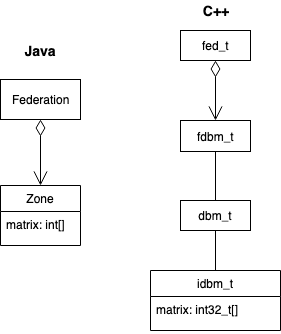
\includegraphics[scale=0.7]{figures/federation.png}
  \caption{Java vs C++ representation of a federation}
  \label{fig:federation}
\end{figure}

\section{Using federations to detect missing intervals}

When performing a refinement check, we must check for the input, output and delay rule. Since refinement is a binary relation, this must be done for each of the pairs belonging to the relation. 

Let (s, t) be the pair consisting of the initial states of the transition systems derived from S and T, shown in Figure \ref{fig:missingIntervals}. Since we have an output transition from s defined for valuations of x in the interval [20, 50], the same should hold for t in order for refinement to hold. However, in the case of t, the output transition is defined only for $[20, 30] \cup [40, 50]$, which means that we need a mechanism for determining that the (30, 40) interval is missing. 

One of our first ideas was to check the minimum and the maximum value for which the transition is enabled. This approach would fail, as the missing interval would not be caught.

An approach that would catch missing intervals is to use subtraction of federations. This involves building a federation with zones corresponding to all edges of a given action for one of the sides and then doing the same thing for the other side. Depending on whether it is an input or an output action, we subtract one federation from the other and if the resulting federation is not empty, then we can conclude that the rule is violated.

\begin{figure}
  \centering
  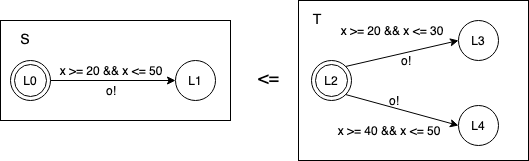
\includegraphics[scale=0.7]{figures/missingIntervals.png}
  \caption{S does not refine T}
  \label{fig:missingIntervals}
\end{figure}

\section{Input-enabledness}

After concluding that each transition system should be a specification by default, we realized the need to treat each state of a transition system as if it was input-enabled.

An automaton like the one in Figure \ref{fig:beforeInputEnabledness} derives a transition system that is not a specification, as not all states are input-enabled. State (L0, \{$x \in [0, \infty)$, $y \in [0, \infty)$\}) can only accept input i1 for values of x and y lower than 10 (included) and input i2 can be taken only for values of x and y higher than 3 (included). Moreover, the states corresponding to locations L1 and L2 do not accept any inputs.

\begin{figure}
  \centering
  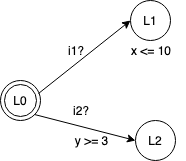
\includegraphics[scale=0.7]{figures/inputEnablednessBefore.png}
  \caption{Automaton resulting in transition system that is not a specification}
  \label{fig:beforeInputEnabledness}
\end{figure}

If we were to modify the previous automaton so that it would derive a specification, it would look like the one in Figure \ref{fig:afterInputEnabledness}. This automaton has all the missing self-loops added to each location, in order to ensure input-enabledness.

\begin{figure}
  \centering
  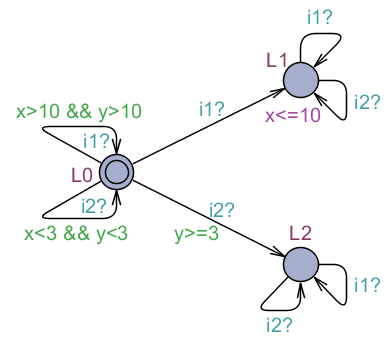
\includegraphics[scale=0.7]{figures/inputEnablednessAfter.png}
  \caption{Automaton resulting in transition system that is a specification}
  \label{fig:afterInputEnabledness}
\end{figure}

We discovered two ways of tackling the issue of input-enabledness: either to add the missing input transitions for each state whenever we try to fetch the next transitions from that state, or to perform the operation of adding the missing input edges to each automaton the moment that it is constructed.

While the former is somewhat easier to implement, the disadvantage is that the action would be repeated each time the next transitions for a state are requested. The latter, on the other hand, is an operation that only needs to be done once and this was a strong reason to choose it. Moreover, to simplify this task, we also opted for adding the invariant of the target location to each edge, as this makes it easier to understand the zone for which a certain input can be received and then derive the missing zones. In case there are resets on the edge, this step is skipped, as the invariant will always be satisfied.

\begin{algorithm}[H]
\caption{Apply input-enabledness function}
\label{alg:apply-input-enabledness}
\begin{algorithmic}[1]
\Function{ApplyInputEnabledness}{}
\ForAll{$loc$ in $locations$}
    \State $zone \gets initializeZone()$
    \State
    \ForAll{$invariant$ in $loc.Invariants$}
        \State $zone.\textsc{buildConstraintsForGuard}(invariant)$
    \EndFor
    \State $fullFederation \gets \{zone\}$
    \State
    \ForAll{$input$ in $inputs$}
        \State $inputEdges \gets \textsc{getEdgesFromLocation}(loc, input)$
        \State $zones \gets \{\}$
        \ForAll{$edge$ in $inputEdges$}
            \State $guardZone \gets zone$
            \ForAll{$guard$ in $edge.Guards$}
                \State $guardZone.\textsc{buildConstraintsForGuard}(guard)$
            \EndFor
            \State add $guardZone$ to $zones$
        \EndFor
        \State
        \State $federation \gets zones$
        \State $resultFederation \gets fullFederation - federation$
        \State
        \ForAll{$zone$ in $edgeZones$}
            \State $newEdge \gets$ (loc, loc, input, \textsc{buildGuardsFromZone}(edgeZone))
            \State add $newEdge$ to $edges$
        \EndFor
    \EndFor
\EndFor
\EndFunction
\end{algorithmic}
\end{algorithm}

Our implementation of the \textsc{ApplyInputEnabledness()} function is shown in Algorithm \ref{alg:apply-input-enabledness}. It starts out by iterating over all locations of an automaton, building a zone with the help of the invariants and using it to construct the federation belonging to that state. Then it looks at all the input edges corresponding to a single action and builds a federation consisting of a zone for each edge. In order to get the missing zones, this federation is subtracted from the full federation built in the beginning. The result of the subtraction is then used to build an edge for each zone and add it to the automaton's edges.

\section{Duplicate automata in refinement query} \label{sec:dupProc}

When running a refinement query, if the same automaton is present more than once on either side of the refinement, then problems can arise. Such a scenario can occur in a self refinement query, but also in more complex queries containing compositions or conjunctions. The main issue that we discovered is in the manipulation of zones, as applying constraints and updates on a clock will do that on the first occurrence of said clock, which is not necessarily the correct occurrence, as the same automaton can appear multiple times.

One solution to this problem would be to make a deep copy of each automaton whenever it is seen, given that it is not its first occurrence. This way we can ensure that the set of clocks of an automaton and the set of clocks of its copy are not the same, so we have a reference to the clock of the right automaton.

Another solution is to display an error message, in the style of \ecdar 0.10, which reports a "Duplicate process instance" error and points to the automaton that appears more than once in the query.

We found both approaches reasonable and estimated that they would require roughly the same time to implement. In order to maintain a consistency between \jecdar and \ecdar wherever it is sensible, we opted for reporting an error message in queries containing duplicate instances of an automaton.

\section{Error logging}

While \ecdar 2.x simply returns "yes", "no" or "maybe" as the result of a query, \ecdar 0.10 provides the user with significantly more feedback, namely it decides whether a query passes or fails, and in case of the latter it displays an error message pointing to the reasons why the chosen query did not succeed. Such messages include stating that there is a duplicate process instance, as presented in Section \ref{sec:dupProc}, or that an automaton is inconsistent.

We believe that offering the user the chance to see why a certain query has failed brings value and can contribute to the construction of correct models. For this reason, error messages were added to \jecdar.

This modification requires the different queries to check for all preconditions instead of terminating when the first issue is encountered. If any of the preconditions fails, then the refinement check is not run and the query fails, as expected. Having to check all preconditions can decrease performance in situations where the first issue is discovered early in the process, however it provides feedback and we think this trade-off is justified in the long run, especially as the size of models increases and they become harder to debug.

Figure \ref{fig:errLog} shows an example of the error messages that \jecdar returns when a query fails.

\begin{figure}
    \centering
    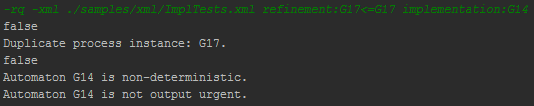
\includegraphics[scale = 0.7]{figures/ErrorMessages.png}
    \caption{Error logging example for multiple queries.}
    \label{fig:errLog}
\end{figure}

\section{Jecdar commands}
As mentioned in \textcite{Jecdar:2019}, we have several commands that can be used for communicating with \jecdar from the terminal. The list of commands can be seen in Table \ref{tbl:commands}. The "-rq folderPath query query..." command, which runs one or more queries, given the path of the model, has been modified with the addition of an extra flag to indicate whether the model is in JSON or in XML format. The reason for doing is so that the controller can decide which parser it should use. In order to run such a command, "-rq" must be typed, followed by either "-json" or "-xml", followed by the actual queries.

An important notice one shall take, that \jecdar is now capable of recognising such keywords as determinism, consistency and implementation. One may simply invoke the "-rq" command and in the query specify that they want to get determinism check results. An example of such query could be "determinism:Machine", running this query will show if the automaton is deterministic.

In \ecdar 0.10 and \ecdar 2.x the determinism check as a stand alone check does not exists, however it is included in the consistency as well implementation checks.
%In addition to the previously mentioned commands, there were introduced two new commands in order to be able to return the Refinement relation as well as Refinement trace if the check return false. Table \ref{tbl:newCommands} provides with the list of new commands added to \jecdar. It is important that one would keep in mind to provide with the corresponding flag, which indicates whether it is JSON or XML format. The "-rqrr" command returns the refinement relation in a tree format as well as the result if it fails or not.

\begin{center}
\begin{table}
    \begin{tabular}{ | l | p{6cm} |}
    \hline
    Commands & Description of commands\\ \hline \hline
\textbf{-help} &This command provides a list of all \jecdar commands as well as their usage\\ 
\hline
\textbf{-version} &Returns the current version of the engine.\\ 
\hline
\textbf{-vq query} &Given a query this command will verify if the query is syntactically correct.\\
\hline

\textbf{-rq -json/-xml folderPath query query...} &Given a folder location with indicator for the format of the files and one or more queries this command will firstly check if the queries are syntactically correct and then will run them.\\ 

\hline
    \end{tabular}
    \caption{\jecdar commands \textcite{Jecdar:2019}}
     \label{tbl:commands}
     \end{table}
\end{center}




\iffalse
\begin{center}
\begin{table}
    \begin{tabular}{ | l | p{5.7cm} |}
    \hline
    Commands & Description of commands\\ \hline \hline
\textbf{-rqrr -json/-xml folderPath query query...} &This command works very alike to -rq, except it returns the refinement relation. Given a folder location with indicator for the format and one or more queries this command will execute the check and return the refinement relation.\\ 
\hline
\textbf{-rqrt -json/-xml folderPath query query...} &This command works almost the same as -rqrr, however instead of returning refinement relation, it will return trace to where the refinement check failed.\\ 
\hline
    \end{tabular}
    \caption{New \jecdar commands}
     \label{tbl:newCommands}
     \end{table}
\end{center}
\fi

